\documentclass[12pt]{article} % use larger type; default would be 10pt

\usepackage{pgfplots}
\usetikzlibrary{calc}
\usetikzlibrary{arrows}
\usetikzlibrary{patterns}
\usetikzlibrary{calc,intersections,through,backgrounds}
\usetikzlibrary{decorations.pathreplacing}
        \usepackage{xcolor} 
        \newcommand\degree[0]{^{\circ}}
        \newcommand\abs[1]{\left|#1\right|}
\usepackage{amsmath}
        \newcommand{\alert}[1]{\boldsymbol{\color{magenta}{#1}}}
        \newcommand{\blert}[1]{\boldsymbol{\color{blue}{#1}}}

\title{Play with TikZ}
\author{Just Us}
%\date{} % Activate to display a given date or no date (if empty),
         % otherwise the current date is printed 

\begin{document}
\maketitle

\section{Chap 6 Section 4}




fig-6-4-ex1

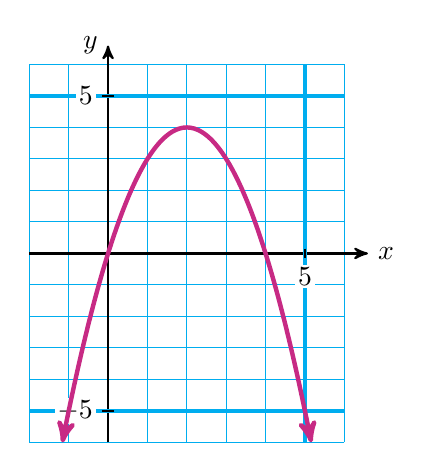
\begin{tikzpicture}[xscale=.5, yscale=.4]
\draw[cyan] (-2,-6) grid (6,6);
\draw[black, thick, ->, >=stealth'] (-2,0)--(6.6,0) node[right]{$x$};
\draw[black, thick, ->, >=stealth'] (0,-6)--(0,6.6) node[left]{$y$};
\foreach \x in {5} {
 \draw[cyan, very thick] (\x,-6)--++(0,12);
 \draw[black, thick] (\x,.15) --++(0,-.3) node[below, yshift=-2, fill=white, inner sep=1]   {$\x$};
}
\foreach \x in  {-5,5} {
 \draw[cyan, very thick] (-2,\x)--++(8,0);
\draw[black, thick] (.15,\x) --++(-.3,0) node[left, xshift=-2, fill=white, inner sep=1]   {$\x$};
}
\draw[samples=65,domain={2-sqrt(10)}:{2+sqrt(10)},smooth,variable=\x,magenta!80!black, ultra thick, <->,>=stealth'] plot ({\x},{4-(\x-2)^2});
\end{tikzpicture}
\newline

fig-6-4-1

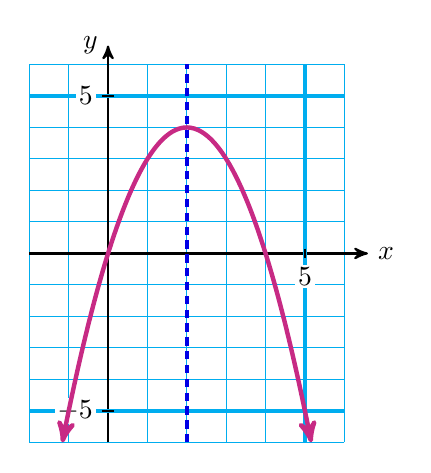
\begin{tikzpicture}[xscale=.5, yscale=.4]
\draw[cyan] (-2,-6) grid (6,6);
\draw[black, thick, ->, >=stealth'] (-2,0)--(6.6,0) node[right]{$x$};
\draw[black, thick, ->, >=stealth'] (0,-6)--(0,6.6) node[left]{$y$};
\foreach \x in {5} {
 \draw[cyan, very thick] (\x,-6)--++(0,12);
 \draw[black, thick] (\x,.15) --++(0,-.3) node[below, yshift=-2, fill=white, inner sep=1]   {$\x$};
}
\foreach \x in  {-5,5} {
 \draw[cyan, very thick] (-2,\x)--++(8,0);
\draw[black, thick] (.15,\x) --++(-.3,0) node[left, xshift=-2, fill=white, inner sep=1]   {$\x$};
}
\draw[samples=65,domain={2-sqrt(10)}:{2+sqrt(10)},smooth,variable=\x,magenta!80!black, ultra thick, <->,>=stealth'] plot ({\x},{4-(\x-2)^2});
\draw[ultra thick, densely dashed,blue!90!black] (2,-6)--(2,6);
\end{tikzpicture}
\newline

sw-6-4-1 grid

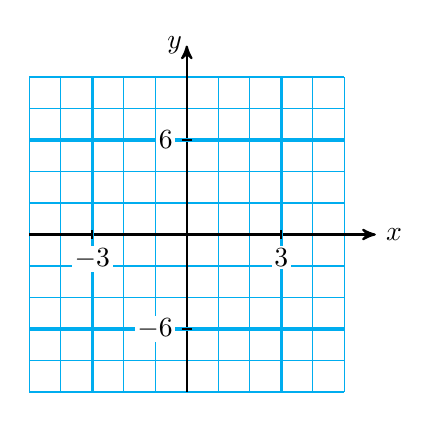
\begin{tikzpicture}[scale=.4]
\draw[cyan] (-5,-5) grid (5,5);
\draw[black, thick, ->, >=stealth'] (-5,0)--(6,0) node[right]{$x$};
\draw[black, thick, ->, >=stealth'] (0,-5)--(0,6) node[left, xshift=2]{$y$};
\foreach \x in {-3,3} {
 \draw[cyan, very thick] (\x,-5)--++(0,10);
 \draw[black, thick] (\x,.15) --++(0,-.3) node[below, yshift=-2, fill=white, inner sep=1]   {$\x$};
}
\foreach \x [evaluate=\x as \xi using int(2*\x)] in  {-3,3} {
 \draw[cyan, very thick] (-5,\x)--++(10,0);
\draw[black, thick] (.15,\x) --++(-.3,0) node[left, xshift=-2, fill=white, inner sep=1]   {$\xi$};
}
\end{tikzpicture}
\newline


sw-6-4-2 grid

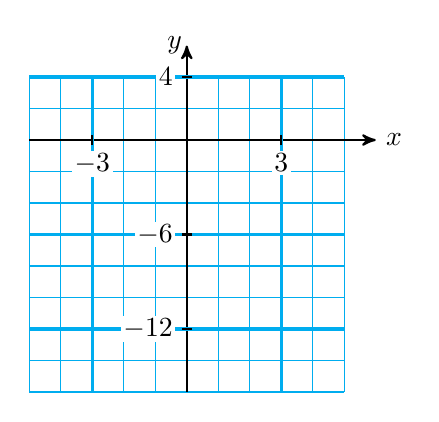
\begin{tikzpicture}[scale=.4]
\draw[cyan] (-5,-8) grid (5,2);
\draw[black, thick, ->, >=stealth'] (-5,0)--(6,0) node[right]{$x$};
\draw[black, thick, ->, >=stealth'] (0,-8)--(0,3) node[left, xshift=2]{$y$};
\foreach \x in {-3,3} {
 \draw[cyan, very thick] (\x,-8)--++(0,10);
 \draw[black, thick] (\x,.15) --++(0,-.3) node[below, yshift=-2, fill=white, inner sep=1]   {$\x$};
}
\foreach \x [evaluate=\x as \xi using int(2*\x)] in  {-3,-6,2} {
 \draw[cyan, very thick] (-5,\x)--++(10,0);
\draw[black, thick] (.15,\x) --++(-.3,0) node[left, xshift=-2, fill=white, inner sep=1]   {$\xi$};
}
\end{tikzpicture}
\newline


sw-6-4-3 grid

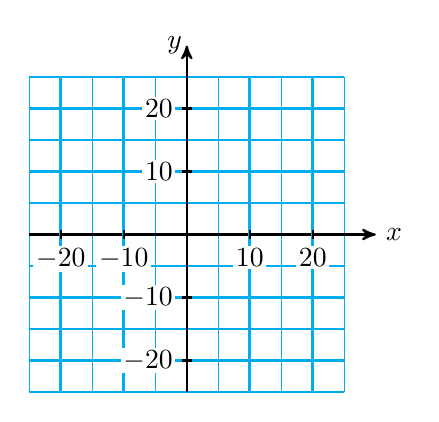
\begin{tikzpicture}[scale=.4]
\draw[cyan] (-5,-5) grid (5,5);
\draw[black, thick, ->, >=stealth'] (-5,0)--(6,0) node[right]{$x$};
\draw[black, thick, ->, >=stealth'] (0,-5)--(0,6) node[left, xshift=2]{$y$};
\foreach \x [evaluate=\x as \xi using int(5*\x)] in {-4,-2,2,4} {
 \draw[cyan, very thick] (\x,-5)--++(0,10);
 \draw[black, thick] (\x,.15) --++(0,-.3) node[below, yshift=-2, fill=white, inner sep=1]   {$\xi$};
}
\foreach \x [evaluate=\x as \xi using int(5*\x)] in  {-4,-2,2,4} {
 \draw[cyan, very thick] (-5,\x)--++(10,0);
\draw[black, thick] (.15,\x) --++(-.3,0) node[left, xshift=-2, fill=white, inner sep=1]   {$\xi$};
}
\end{tikzpicture}
\newline


sw-6-4-4 grid

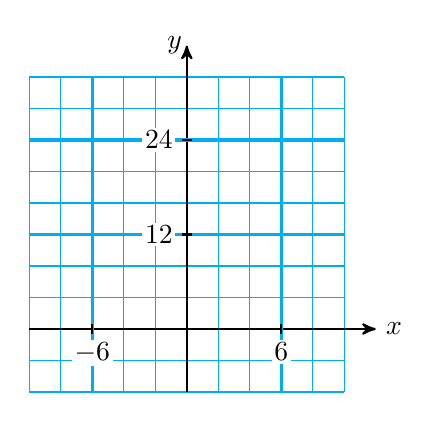
\begin{tikzpicture}[scale=.4]
\draw[cyan] (-5,-2) grid (5,8);
\draw[black, thick, ->, >=stealth'] (-5,0)--(6,0) node[right]{$x$};
\draw[black, thick, ->, >=stealth'] (0,-2)--(0,9) node[left, xshift=2]{$y$};
\foreach \x [evaluate=\x as \xi using int(2*\x)] in {-3,3} {
 \draw[cyan, very thick] (\x,-2)--++(0,10);
 \draw[black, thick] (\x,.15) --++(0,-.3) node[below, yshift=-2, fill=white, inner sep=1]   {$\xi$};
}
\foreach \x [evaluate=\x as \xi using int(4*\x)] in  {3,6} {
 \draw[cyan, very thick] (-5,\x)--++(10,0);
\draw[black, thick] (.15,\x) --++(-.3,0) node[left, xshift=-2, fill=white, inner sep=1]   {$\xi$};
}
\end{tikzpicture}
\newline


hp-6-4-4 grid

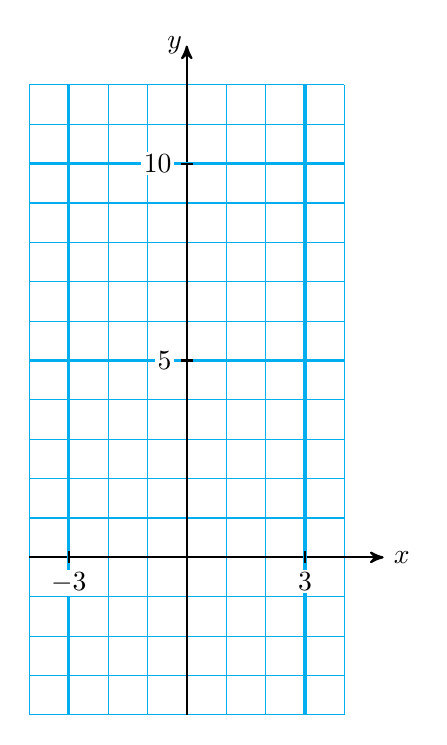
\begin{tikzpicture}[scale=.5]
\draw[cyan] (-4,-4) grid (4,12);
\draw[black, thick, ->, >=stealth'] (-4,0)--(5,0) node[right]{$x$};
\draw[black, thick, ->, >=stealth'] (0,-4)--(0,13) node[left, xshift=2]{$y$};
\foreach \x in {-3,3} {
 \draw[cyan, very thick] (\x,-4)--++(0,16);
 \draw[black, thick] (\x,.15) --++(0,-.3) node[below, yshift=-2, fill=white, inner sep=1]   {$\x$};
}
\foreach \x in  {5,10} {
 \draw[cyan, very thick] (-4,\x)--++(8,0);
\draw[black, thick] (.15,\x) --++(-.3,0) node[left, xshift=-2, fill=white, inner sep=1]   {$\x$};
}
\end{tikzpicture}
\newline


hp-6-4-5 grid

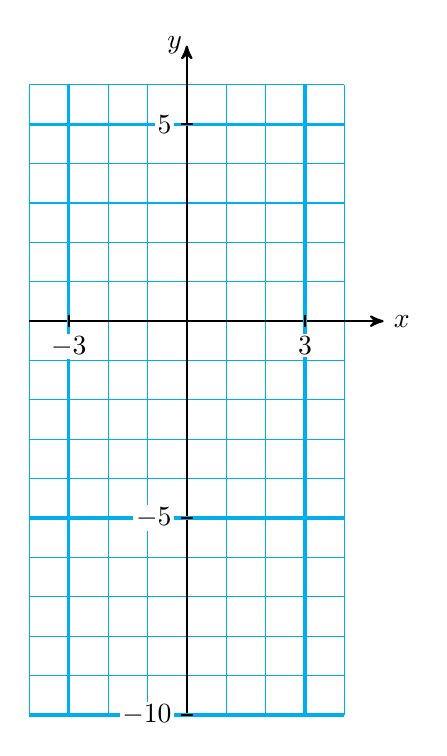
\begin{tikzpicture}[scale=.5]
\draw[cyan] (-4,-10) grid (4,6);
\draw[black, thick, ->, >=stealth'] (-4,0)--(5,0) node[right]{$x$};
\draw[black, thick, ->, >=stealth'] (0,-10)--(0,7) node[left, xshift=2]{$y$};
\foreach \x in {-3,3} {
 \draw[cyan, very thick] (\x,-10)--++(0,16);
 \draw[black, thick] (\x,.15) --++(0,-.3) node[below, yshift=-2, fill=white, inner sep=1]   {$\x$};
}
\foreach \x in  {-5,-10,5} {
 \draw[cyan, very thick] (-4,\x)--++(8,0);
\draw[black, thick] (.15,\x) --++(-.3,0) node[left, xshift=-2, fill=white, inner sep=1]   {$\x$};
}
\end{tikzpicture}
\newline


hp-6-4-5ans parabolas

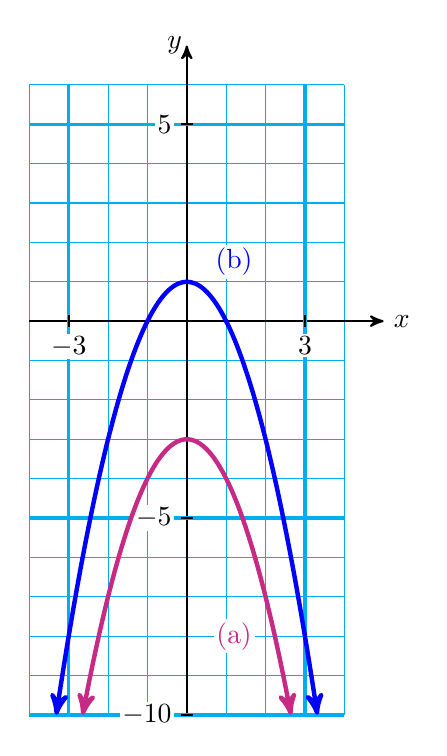
\begin{tikzpicture}[scale=.5]
\draw[cyan] (-4,-10) grid (4,6);
\draw[black, thick, ->, >=stealth'] (-4,0)--(5,0) node[right]{$x$};
\draw[black, thick, ->, >=stealth'] (0,-10)--(0,7) node[left, xshift=2]{$y$};
\foreach \x in {-3,3} {
 \draw[cyan, very thick] (\x,-10)--++(0,16);
 \draw[black, thick] (\x,.15) --++(0,-.3) node[below, yshift=-2, fill=white, inner sep=1]   {$\x$};
}
\foreach \x in  {-5,-10,5} {
 \draw[cyan, very thick] (-4,\x)--++(8,0);
\draw[black, thick] (.15,\x) --++(-.3,0) node[left, xshift=-2, fill=white, inner sep=1]   {$\x$};
}
\draw[samples=65,domain={-sqrt(7)}:{sqrt(7)},smooth,variable=\x,magenta!80!black, ultra thick, <->, >=stealth'] plot ({\x},{-(\x)^2-3});
\node[text=magenta!80!black, fill=white, inner sep=1] at (1.2,-8) {(a)};
\draw[samples=65,domain={-sqrt(11)}:{sqrt(11)},smooth,variable=\x,blue, ultra thick, <->, >=stealth'] plot ({\x},{1-(\x)^2});
\node[text=blue, fill=white, inner sep=1] at (1.2,1.5) {(b)};
\end{tikzpicture}
\newline


hp-6-4-7 grid

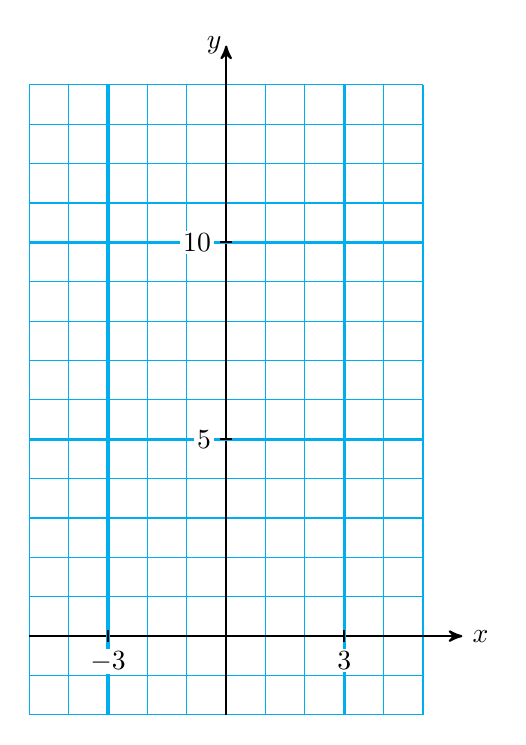
\begin{tikzpicture}[scale=.5]
\draw[cyan] (-5,-2) grid (5,14);
\draw[black, thick, ->, >=stealth'] (-5,0)--(6,0) node[right]{$x$};
\draw[black, thick, ->, >=stealth'] (0,-2)--(0,15) node[left, xshift=2]{$y$};
\foreach \x in {-3,3} {
 \draw[cyan, very thick] (\x,-2)--++(0,16);
 \draw[black, thick] (\x,.15) --++(0,-.3) node[below, yshift=-2, fill=white, inner sep=1]   {$\x$};
}
\foreach \x in  {5,10} {
 \draw[cyan, very thick] (-5,\x)--++(10,0);
\draw[black, thick] (.15,\x) --++(-.3,0) node[left, xshift=-2, fill=white, inner sep=1]   {$\x$};
}
\end{tikzpicture}
\newline


hp-6-4-7ans parabola

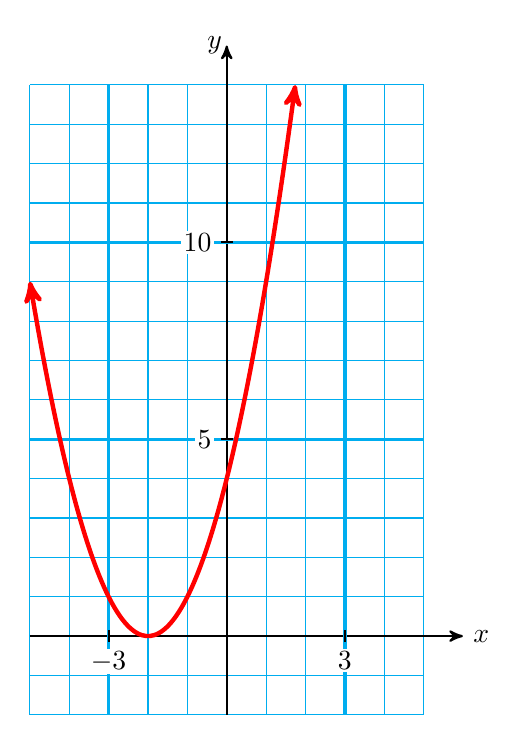
\begin{tikzpicture}[scale=.5]
\draw[cyan] (-5,-2) grid (5,14);
\draw[black, thick, ->, >=stealth'] (-5,0)--(6,0) node[right]{$x$};
\draw[black, thick, ->, >=stealth'] (0,-2)--(0,15) node[left, xshift=2]{$y$};
\foreach \x in {-3,3} {
 \draw[cyan, very thick] (\x,-2)--++(0,16);
 \draw[black, thick] (\x,.15) --++(0,-.3) node[below, yshift=-2, fill=white, inner sep=1]   {$\x$};
}
\foreach \x in  {5,10} {
 \draw[cyan, very thick] (-5,\x)--++(10,0);
\draw[black, thick] (.15,\x) --++(-.3,0) node[left, xshift=-2, fill=white, inner sep=1]   {$\x$};
}
\draw[samples=65,domain={-5}:{-2+sqrt(14)},smooth,variable=\x,red, ultra thick, <->, >=stealth'] plot ({\x},{(\x+2)^2});
\end{tikzpicture}
\newline


hp-6-4-9 5-by-5 grid

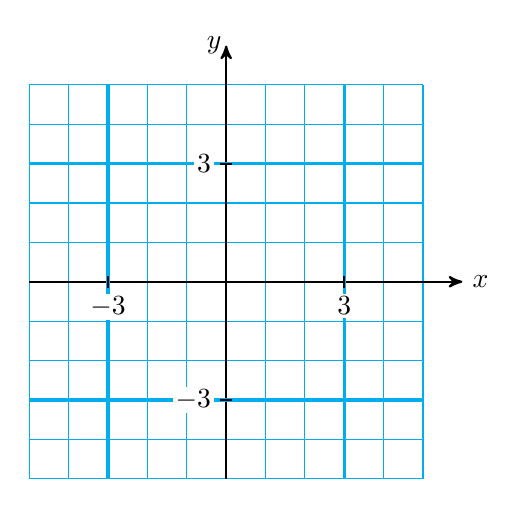
\begin{tikzpicture}[scale=.5]
\draw[cyan] (-5,-5) grid (5,5);
\draw[black, thick, ->, >=stealth'] (-5,0)--(6,0) node[right]{$x$};
\draw[black, thick, ->, >=stealth'] (0,-5)--(0,6) node[left, xshift=2]{$y$};
\foreach \x in {-3,3} {
 \draw[cyan, very thick] (\x,-5)--++(0,10);
 \draw[black, thick] (\x,.15) --++(0,-.3) node[below, yshift=-2, fill=white, inner sep=1]   {$\x$};
}
\foreach \x in  {-3,3} {
 \draw[cyan, very thick] (-5,\x)--++(10,0);
\draw[black, thick] (.15,\x) --++(-.3,0) node[left, xshift=-2, fill=white, inner sep=1]   {$\x$};
}
\end{tikzpicture}
\newline


hp-6-4-9ans parabola

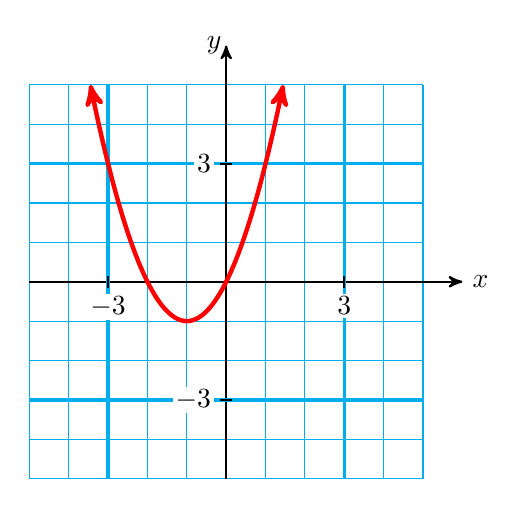
\begin{tikzpicture}[scale=.5]
\draw[cyan] (-5,-5) grid (5,5);
\draw[black, thick, ->, >=stealth'] (-5,0)--(6,0) node[right]{$x$};
\draw[black, thick, ->, >=stealth'] (0,-5)--(0,6) node[left, xshift=2]{$y$};
\foreach \x in {-3,3} {
 \draw[cyan, very thick] (\x,-5)--++(0,10);
 \draw[black, thick] (\x,.15) --++(0,-.3) node[below, yshift=-2, fill=white, inner sep=1]   {$\x$};
}
\foreach \x in  {-3,3} {
 \draw[cyan, very thick] (-5,\x)--++(10,0);
\draw[black, thick] (.15,\x) --++(-.3,0) node[left, xshift=-2, fill=white, inner sep=1]   {$\x$};
}
\draw[samples=65,domain={-sqrt(6)-1}:{sqrt(6)-1},smooth,variable=\x,red, ultra thick, <->, >=stealth'] plot ({\x},{(\x)^2+2*\x});
\end{tikzpicture}
\newline


hp-6-4-11 grid

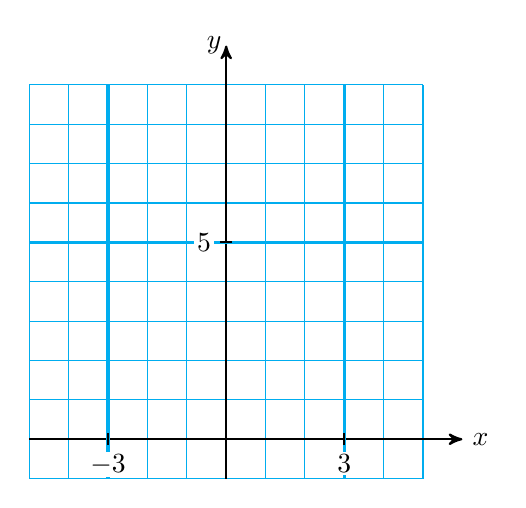
\begin{tikzpicture}[scale=.5]
\draw[cyan] (-5,-1) grid (5,9);
\draw[black, thick, ->, >=stealth'] (-5,0)--(6,0) node[right]{$x$};
\draw[black, thick, ->, >=stealth'] (0,-1)--(0,10) node[left, xshift=2]{$y$};
\foreach \x in {-3,3} {
 \draw[cyan, very thick] (\x,-1)--++(0,10);
 \draw[black, thick] (\x,.15) --++(0,-.3) node[below, yshift=-2, fill=white, inner sep=1]   {$\x$};
}
\foreach \x in  {5} {
 \draw[cyan, very thick] (-5,\x)--++(10,0);
\draw[black, thick] (.15,\x) --++(-.3,0) node[left, xshift=-2, fill=white, inner sep=1]   {$\x$};
}
\end{tikzpicture}
\newline


hp-6-4-11ans parabola

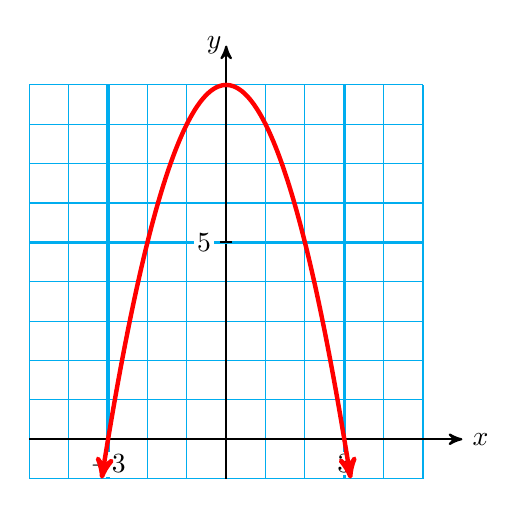
\begin{tikzpicture}[scale=.5]
\draw[cyan] (-5,-1) grid (5,9);
\draw[black, thick, ->, >=stealth'] (-5,0)--(6,0) node[right]{$x$};
\draw[black, thick, ->, >=stealth'] (0,-1)--(0,10) node[left, xshift=2]{$y$};
\foreach \x in {-3,3} {
 \draw[cyan, very thick] (\x,-1)--++(0,10);
 \draw[black, thick] (\x,.15) --++(0,-.3) node[below, yshift=-2, fill=white, inner sep=1]   {$\x$};
}
\foreach \x in  {5} {
 \draw[cyan, very thick] (-5,\x)--++(10,0);
\draw[black, thick] (.15,\x) --++(-.3,0) node[left, xshift=-2, fill=white, inner sep=1]   {$\x$};
}
\draw[samples=65,domain={-sqrt(10)}:{sqrt(10)},smooth,variable=\x,red, ultra thick, <->, >=stealth'] plot ({\x},{9-(\x)^2});
\end{tikzpicture}
\newline


hp-6-4-13ans parabolas

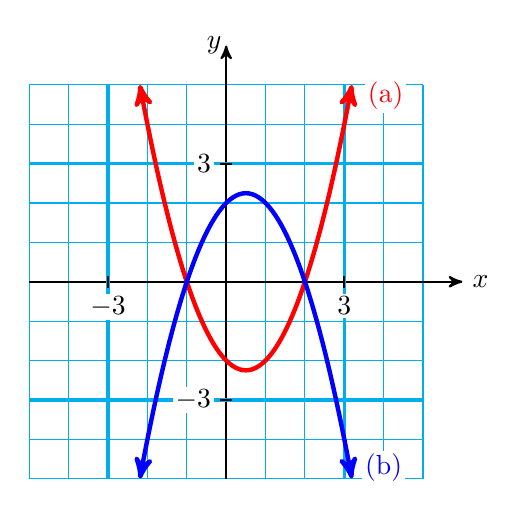
\begin{tikzpicture}[scale=.5]
\draw[cyan] (-5,-5) grid (5,5);
\draw[black, thick, ->, >=stealth'] (-5,0)--(6,0) node[right]{$x$};
\draw[black, thick, ->, >=stealth'] (0,-5)--(0,6) node[left, xshift=2]{$y$};
\foreach \x in {-3,3} {
 \draw[cyan, very thick] (\x,-5)--++(0,10);
 \draw[black, thick] (\x,.15) --++(0,-.3) node[below, yshift=-2, fill=white, inner sep=1]   {$\x$};
}
\foreach \x in  {-3,3} {
 \draw[cyan, very thick] (-5,\x)--++(10,0);
\draw[black, thick] (.15,\x) --++(-.3,0) node[left, xshift=-2, fill=white, inner sep=1]   {$\x$};
}
\draw[samples=65,domain={-sqrt(29)/2+1/2}:{sqrt(29)/2+1/2},smooth,variable=\x,red, ultra thick, <->, >=stealth'] plot ({\x},{(\x)^2-\x-2}) node[right, xshift=4, yshift=-4, fill=white, inner sep=1]{(a)};
\draw[samples=65,domain={-sqrt(29)/2+1/2}:{sqrt(29)/2+1/2},smooth,variable=\x,blue, ultra thick, <->, >=stealth'] plot ({\x},{-(\x)^2+\x+2}) node[right, xshift=3, yshift=4, fill=white, inner sep=1]{(b)};
\end{tikzpicture}
\newline


hp-6-4-14 grid

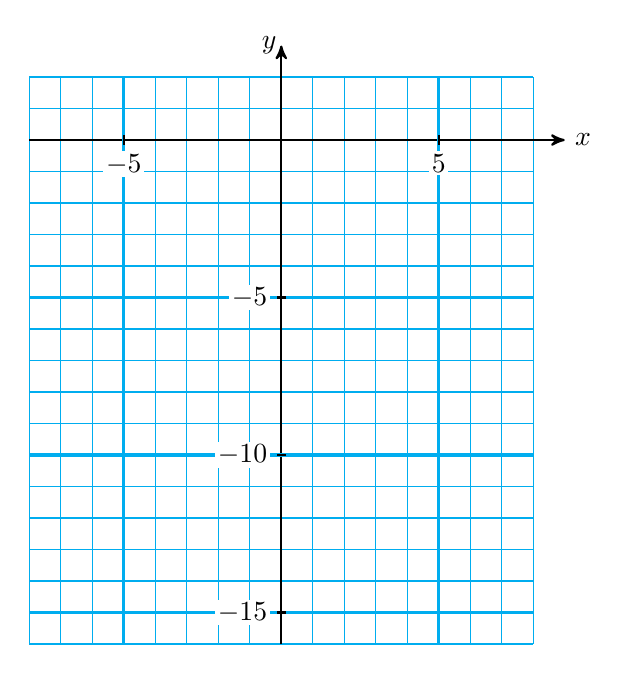
\begin{tikzpicture}[scale=.4]
\draw[cyan] (-8,-16) grid (8,2);
\draw[black, thick, ->, >=stealth'] (-8,0)--(9,0) node[right]{$x$};
\draw[black, thick, ->, >=stealth'] (0,-16)--(0,3) node[left, xshift=2]{$y$};
\foreach \x in {-5,5} {
 \draw[cyan, very thick] (\x,-16)--++(0,18);
 \draw[black, thick] (\x,.15) --++(0,-.3) node[below, yshift=-2, fill=white, inner sep=1]   {$\x$};
}
\foreach \x in  {-15,-10,-5} {
 \draw[cyan, very thick] (-8,\x)--++(16,0);
\draw[black, thick] (.15,\x) --++(-.3,0) node[left, xshift=-2, fill=white, inner sep=1]   {$\x$};
}
\end{tikzpicture}
\newline


hp-6-4-15 grid

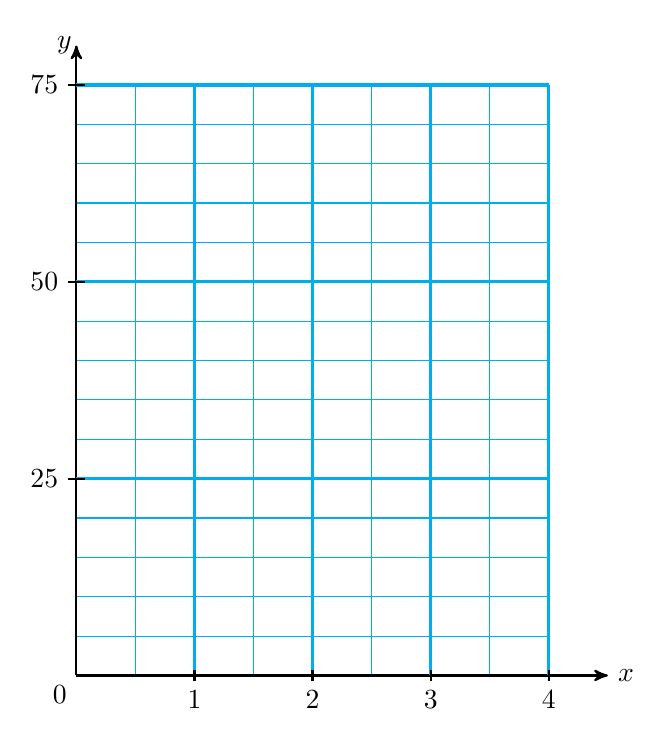
\begin{tikzpicture}[xscale=.75, yscale=.5]
\draw[cyan] (0,0) grid (8,15);
\draw[black, thick, ->, >=stealth'] (0,0)--(9,0) node[right]{$x$};
\draw[black, thick, ->, >=stealth'] (0,0)--(0,16) node[left, xshift=2]{$y$};
\foreach \x [evaluate=\x as \xi using int(.5*\x)] in {2,4,6,8} {
 \draw[cyan, very thick] (\x,0)--++(0,15);
 \draw[black, thick] (\x,.15) --++(0,-.3) node[below, yshift=-2, fill=white, inner sep=1]   {$\xi$};
}
\foreach \x [evaluate=\x as \xi using int(5*\x)] in  {5,10,15} {
 \draw[cyan, very thick] (0,\x)--++(8,0);
\draw[black, thick] (.15,\x) --++(-.3,0) node[left, xshift=-2, fill=white, inner sep=1]   {$\xi$};
}
\node[below left] at (0,0) {$0$};
\end{tikzpicture}
\newline


hp-6-4-15ans parabola

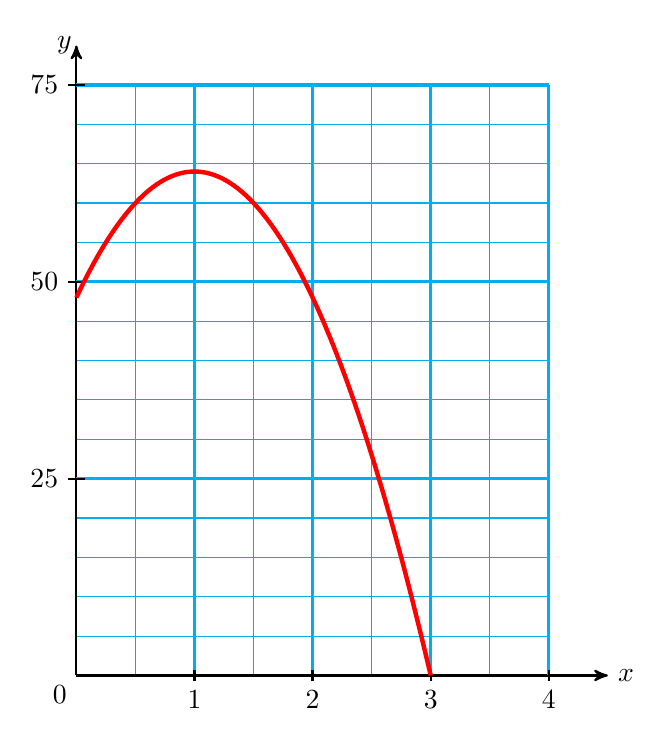
\begin{tikzpicture}[xscale=.75, yscale=.5]
\draw[cyan] (0,0) grid (8,15);
\draw[black, thick, ->, >=stealth'] (0,0)--(9,0) node[right]{$x$};
\draw[black, thick, ->, >=stealth'] (0,0)--(0,16) node[left, xshift=2]{$y$};
\foreach \x [evaluate=\x as \xi using int(.5*\x)] in {2,4,6,8} {
 \draw[cyan, very thick] (\x,0)--++(0,15);
 \draw[black, thick] (\x,.15) --++(0,-.3) node[below, yshift=-2, fill=white, inner sep=1]   {$\xi$};
}
\foreach \x [evaluate=\x as \xi using int(5*\x)] in  {5,10,15} {
 \draw[cyan, very thick] (0,\x)--++(8,0);
\draw[black, thick] (.15,\x) --++(-.3,0) node[left, xshift=-2, fill=white, inner sep=1]   {$\xi$};
}
\node[below left] at (0,0) {$0$};
\draw[samples=65,domain=0:{3},smooth,variable=\x,red, ultra thick] plot ({2*\x},{(48+32*\x-16*(\x)^2)/5});
\end{tikzpicture}
\newline

\section{Section 6.5}



fig-6-5-1 parabola

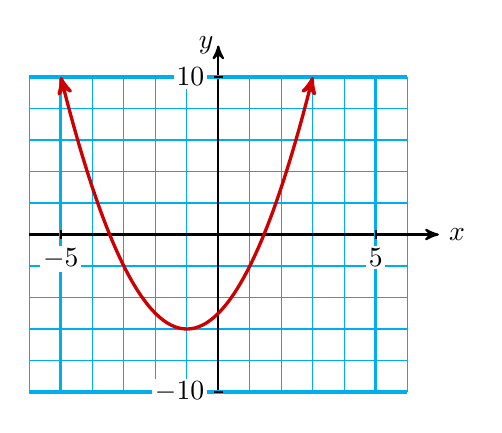
\begin{tikzpicture}[scale=.4]
\draw[cyan] (-6,-5) grid (6,5);
\draw[black, thick, ->, >=stealth'] (-6,0)--(7,0) node[right]{$x$};
\draw[black, thick, ->, >=stealth'] (0,-5)--(0,6) node[left, xshift=2]{$y$};
\foreach \x  in {-5,5} {
 \draw[cyan, very thick] (\x,-5)--++(0,10);
 \draw[black, thick] (\x,.15) --++(0,-.3) node[below, yshift=-2, fill=white, inner sep=1]   {$\x$};
}
\foreach \x [evaluate=\x as \xi using int(2*\x)] in  {-5,5} {
 \draw[cyan, very thick] (-6,\x)--++(12,0);
\draw[black, thick] (.15,\x) --++(-.3,0) node[left, xshift=-2, fill=white, inner sep=1]   {$\xi$};
}
\draw[samples=65,domain=-5:3,smooth,variable=\x,red!80!black, very thick, <->, >=stealth'] plot ({\x},{((\x)^2 +2*\x-5)/2});
\end{tikzpicture}
\newline



fig-6-5-2 parabola with no x-intercepts

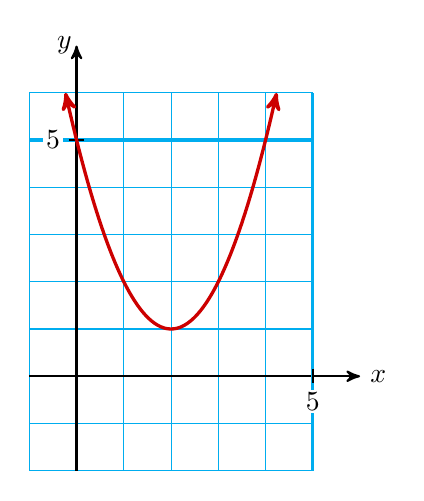
\begin{tikzpicture}[scale=.6]
\draw[cyan] (-1,-2) grid (5,6);
\draw[black, thick, ->, >=stealth'] (-1,0)--(6,0) node[right]{$x$};
\draw[black, thick, ->, >=stealth'] (0,-2)--(0,7) node[left, xshift=2]{$y$};
\foreach \x  in {5} {
 \draw[cyan, very thick] (\x,-2)--++(0,8);
 \draw[black, thick] (\x,.15) --++(0,-.3) node[below, yshift=-2, fill=white, inner sep=1]   {$\x$};
}
\foreach \x in  {5} {
 \draw[cyan, very thick] (-1,\x)--++(6,0);
\draw[black, thick] (.15,\x) --++(-.3,0) node[left, xshift=-2, fill=white, inner sep=1]   {$\x$};
}
\draw[samples=65,domain={2-sqrt(5)}:{2+sqrt(5)},smooth,variable=\x,red!80!black, very thick, <->, >=stealth'] plot (\x,{((\x-2)^2 +1});
\end{tikzpicture}
\newline


hp-6-5-15 triangle

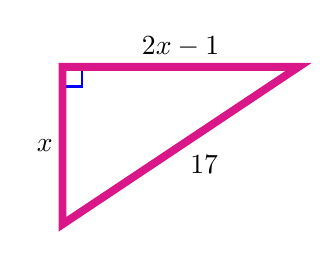
\begin{tikzpicture}
\draw[blue,thick] (0,0) rectangle ++(.25,-.25);
\draw[magenta!90!black, line width=1mm] (0,0)--(3,0)--(0,-2)--cycle;
\node[left] at (0,-1) {$x$};
\node[above] at (1.5,0) {$2x-1$};
\node[below right] at (1.5,-1) {$17$};
\end{tikzpicture}
\newline


hp-6-5-16 triangle

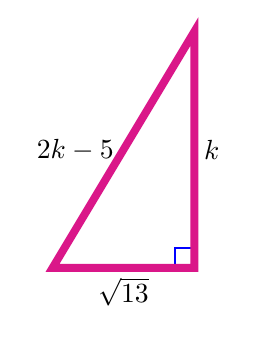
\begin{tikzpicture}
\draw[blue,thick] (0,0) rectangle ++(-.25,.25);
\draw[magenta!90!black, line width=1mm] (0,0)--(-1.8,0)--(0,3)--cycle;
\node[right] at (0,1.5) {$k$};
\node[below] at (-.9,0) {$\sqrt{13}$};
\node[left] at (-.9,1.5) {$2k-5$};
\end{tikzpicture}
\newline


hp-6-5-17ans parabola

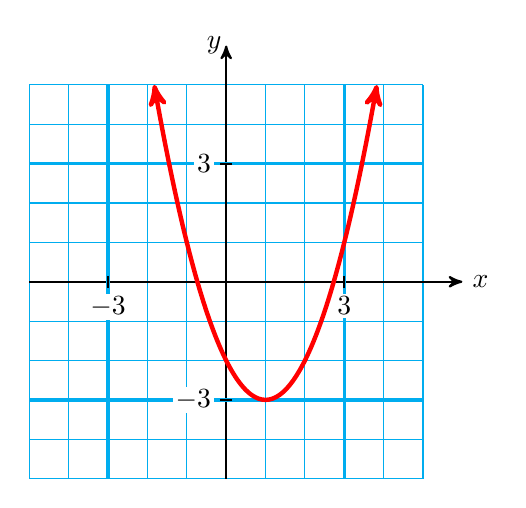
\begin{tikzpicture}[scale=.5]
\draw[cyan] (-5,-5) grid (5,5);
\draw[black, thick, ->, >=stealth'] (-5,0)--(6,0) node[right]{$x$};
\draw[black, thick, ->, >=stealth'] (0,-5)--(0,6) node[left, xshift=2]{$y$};
\foreach \x in {-3,3} {
 \draw[cyan, very thick] (\x,-5)--++(0,10);
 \draw[black, thick] (\x,.15) --++(0,-.3) node[below, yshift=-2, fill=white, inner sep=1]   {$\x$};
}
\foreach \x in  {-3,3} {
 \draw[cyan, very thick] (-5,\x)--++(10,0);
\draw[black, thick] (.15,\x) --++(-.3,0) node[left, xshift=-2, fill=white, inner sep=1]   {$\x$};
}
\draw[samples=65,domain={-sqrt(8)+1}:{sqrt(8)+1},smooth,variable=\x,red, ultra thick, <->, >=stealth'] plot ({\x},{(\x)^2-2*\x-2});
\end{tikzpicture}
\newline


hp-6-5-18 5-by-5 grid

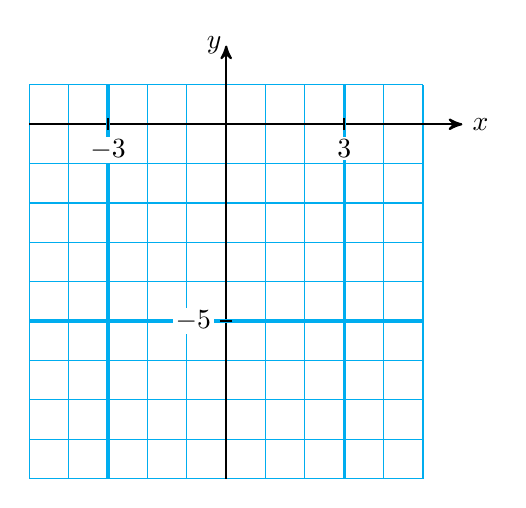
\begin{tikzpicture}[scale=.5]
\draw[cyan] (-5,-9) grid (5,1);
\draw[black, thick, ->, >=stealth'] (-5,0)--(6,0) node[right]{$x$};
\draw[black, thick, ->, >=stealth'] (0,-9)--(0,2) node[left, xshift=2]{$y$};
\foreach \x in {-3,3} {
 \draw[cyan, very thick] (\x,-9)--++(0,10);
 \draw[black, thick] (\x,.15) --++(0,-.3) node[below, yshift=-2, fill=white, inner sep=1]   {$\x$};
}
\foreach \x in  {-5} {
 \draw[cyan, very thick] (-5,\x)--++(10,0);
\draw[black, thick] (.15,\x) --++(-.3,0) node[left, xshift=-2, fill=white, inner sep=1]   {$\x$};
}
\end{tikzpicture}
\newline


hp-6-5-19 5-by-5 grid 

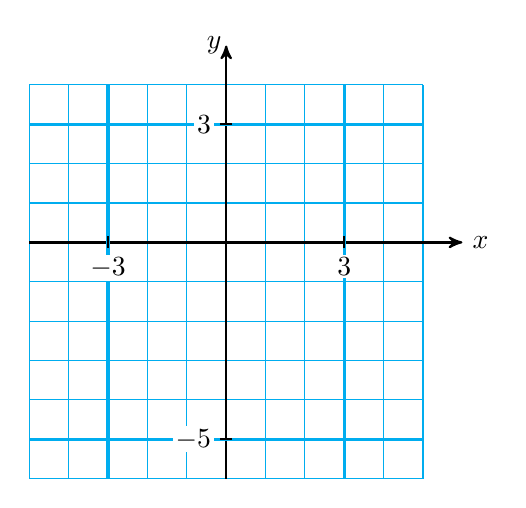
\begin{tikzpicture}[scale=.5]
\draw[cyan] (-5,-6) grid (5,4);
\draw[black, thick, ->, >=stealth'] (-5,0)--(6,0) node[right]{$x$};
\draw[black, thick, ->, >=stealth'] (0,-6)--(0,5) node[left, xshift=2]{$y$};
\foreach \x in {-3,3} {
 \draw[cyan, very thick] (\x,-6)--++(0,10);
 \draw[black, thick] (\x,.15) --++(0,-.3) node[below, yshift=-2, fill=white, inner sep=1]   {$\x$};
}
\foreach \x in  {-5,3} {
 \draw[cyan, very thick] (-5,\x)--++(10,0);
\draw[black, thick] (.15,\x) --++(-.3,0) node[left, xshift=-2, fill=white, inner sep=1]   {$\x$};
}
\end{tikzpicture}
\newline


hp-6-5-19ans parabola 

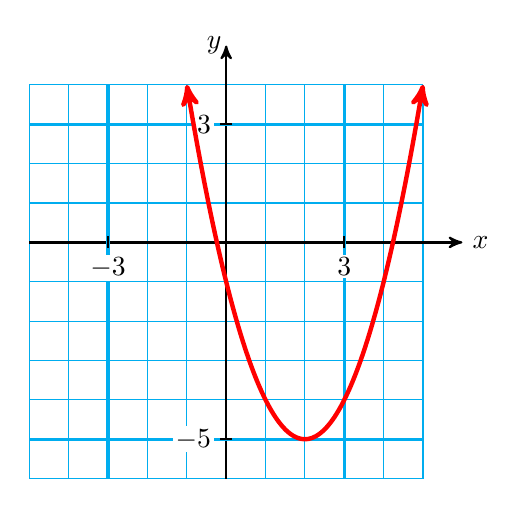
\begin{tikzpicture}[scale=.5]
\draw[cyan] (-5,-6) grid (5,4);
\draw[black, thick, ->, >=stealth'] (-5,0)--(6,0) node[right]{$x$};
\draw[black, thick, ->, >=stealth'] (0,-6)--(0,5) node[left, xshift=2]{$y$};
\foreach \x in {-3,3} {
 \draw[cyan, very thick] (\x,-6)--++(0,10);
 \draw[black, thick] (\x,.15) --++(0,-.3) node[below, yshift=-2, fill=white, inner sep=1]   {$\x$};
}
\foreach \x in  {-5,3} {
 \draw[cyan, very thick] (-5,\x)--++(10,0);
\draw[black, thick] (.15,\x) --++(-.3,0) node[left, xshift=-2, fill=white, inner sep=1]   {$\x$};
}
\draw[samples=65,domain={-1}:{5},smooth,variable=\x,red, ultra thick, <->, >=stealth'] plot ({\x},{(\x)^2-4*\x-1});
\end{tikzpicture}
\newline


cr6-39 grid

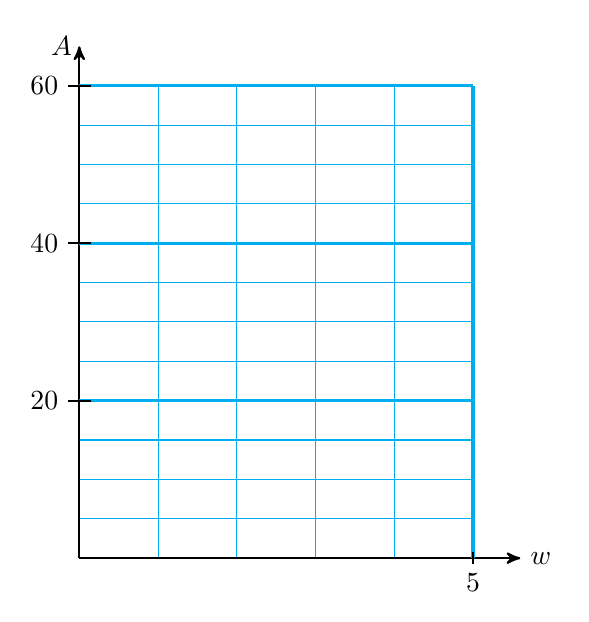
\begin{tikzpicture}[yscale=.5]
\draw[cyan] (0,0) grid (5,12);
\draw[black, thick, ->, >=stealth'] (0,0)--(5.6,0) node[right]{$w$};
\draw[black, thick, ->, >=stealth'] (0,0)--(0,13) node[left, xshift=1]{$A$};
\foreach \x in {5} {
 \draw[cyan, very thick] (\x,0)--++(0,12);
 \draw[black, thick] (\x,.15) --++(0,-.3) node[below, yshift=-2, fill=white, inner sep=1]   {$\x$};
}
\foreach \x [evaluate=\x as \xi using int(5*\x)] in  {4,8,12} {
 \draw[cyan, very thick] (0,\x)--++(5,0);
\draw[black, thick] (.15,\x) --++(-.3,0) node[left, xshift=-2, fill=white, inner sep=1]   {$\xi$};
}
\end{tikzpicture}
\newline


cr6-39ans parabola

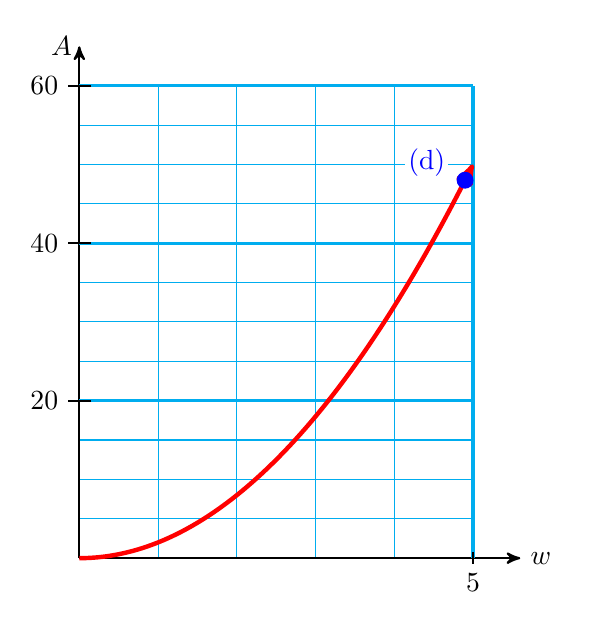
\begin{tikzpicture}[yscale=.5]
\draw[cyan] (0,0) grid (5,12);
\draw[black, thick, ->, >=stealth'] (0,0)--(5.6,0) node[right]{$w$};
\draw[black, thick, ->, >=stealth'] (0,0)--(0,13) node[left, xshift=1]{$A$};
\foreach \x in {5} {
 \draw[cyan, very thick] (\x,0)--++(0,12);
 \draw[black, thick] (\x,.15) --++(0,-.3) node[below, yshift=-2, fill=white, inner sep=1]   {$\x$};
}
\foreach \x [evaluate=\x as \xi using int(5*\x)] in  {4,8,12} {
 \draw[cyan, very thick] (0,\x)--++(5,0);
\draw[black, thick] (.15,\x) --++(-.3,0) node[left, xshift=-2, fill=white, inner sep=1]   {$\xi$};
}
\draw[samples=65,domain=0:{5},smooth,variable=\x,red, ultra thick, ->, >=stealth'] plot ({\x},{0.4*(\x)^2});
\filldraw[blue] ({sqrt(24)}, 48/5) ellipse (1mm and 2mm) node[above left, xshift=-6, fill=white, inner sep=1] {(d)};
\end{tikzpicture}
\newline


cr6-40 grid

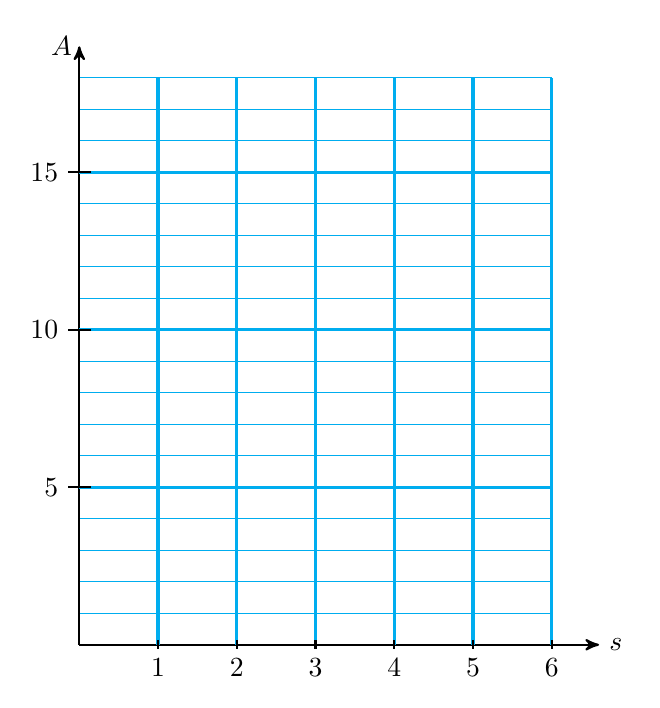
\begin{tikzpicture}[yscale=.4]
\draw[cyan] (0,0) grid (6,18);
\draw[black, thick, ->, >=stealth'] (0,0)--(6.6,0) node[right]{$s$};
\draw[black, thick, ->, >=stealth'] (0,0)--(0,19) node[left, xshift=1]{$A$};
\foreach \x in {1,2,3,...,6} {
 \draw[cyan, very thick] (\x,0)--++(0,18);
 \draw[black, thick] (\x,.15) --++(0,-.3) node[below, yshift=-2, fill=white, inner sep=1]   {$\x$};
}
\foreach \x in  {5,10,15} {
 \draw[cyan, very thick] (0,\x)--++(6,0);
\draw[black, thick] (.15,\x) --++(-.3,0) node[left, xshift=-2, fill=white, inner sep=1]   {$\x$};
}
\end{tikzpicture}
\newline


cr6-41  grid 

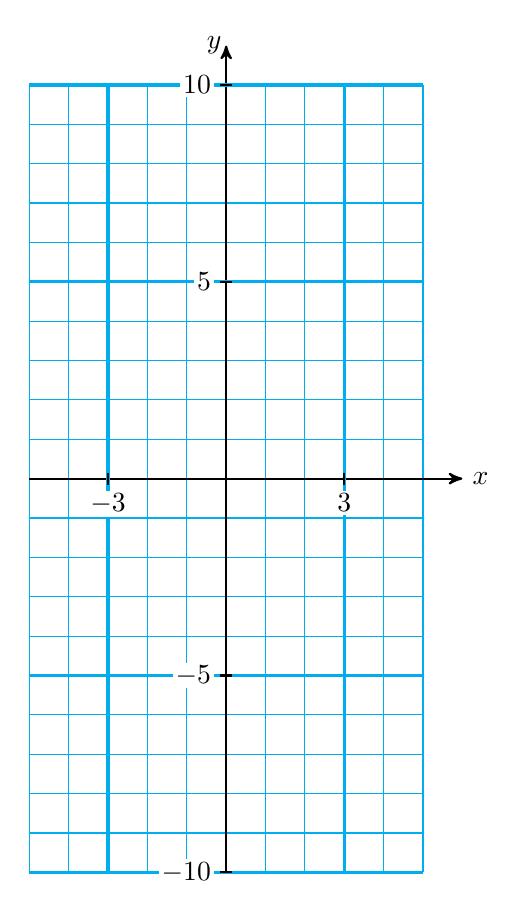
\begin{tikzpicture}[scale=.5]
\draw[cyan] (-5,-10) grid (5,10);
\draw[black, thick, ->, >=stealth'] (-5,0)--(6,0) node[right]{$x$};
\draw[black, thick, ->, >=stealth'] (0,-10)--(0,11) node[left, xshift=2]{$y$};
\foreach \x in {-3,3} {
 \draw[cyan, very thick] (\x,-10)--++(0,20);
 \draw[black, thick] (\x,.15) --++(0,-.3) node[below, yshift=-2, fill=white, inner sep=1]   {$\x$};
}
\foreach \x in  {-10,-5,5,10} {
 \draw[cyan, very thick] (-5,\x)--++(10,0);
\draw[black, thick] (.15,\x) --++(-.3,0) node[left, xshift=-2, fill=white, inner sep=1]   {$\x$};
}
\end{tikzpicture}
\newline


cr6-41ans

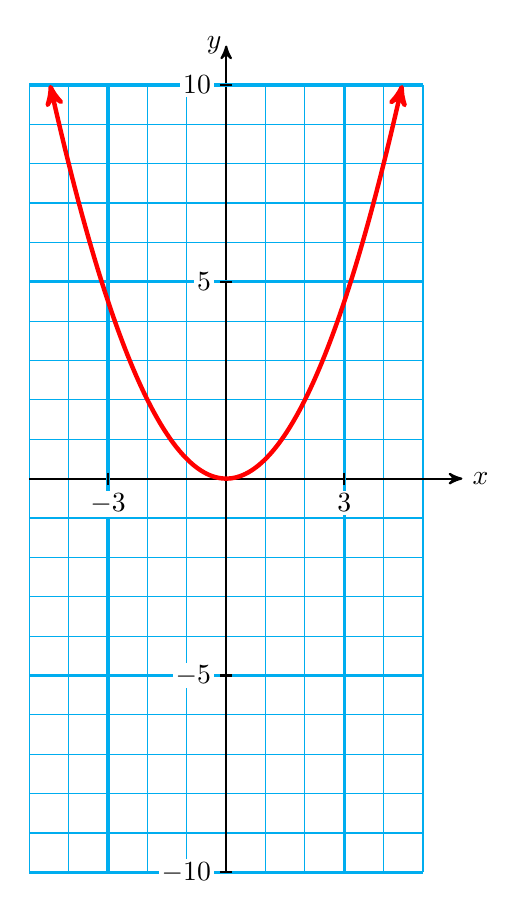
\begin{tikzpicture}[scale=.5]
\draw[cyan] (-5,-10) grid (5,10);
\draw[black, thick, ->, >=stealth'] (-5,0)--(6,0) node[right]{$x$};
\draw[black, thick, ->, >=stealth'] (0,-10)--(0,11) node[left, xshift=2]{$y$};
\foreach \x in {-3,3} {
 \draw[cyan, very thick] (\x,-10)--++(0,20);
 \draw[black, thick] (\x,.15) --++(0,-.3) node[below, yshift=-2, fill=white, inner sep=1]   {$\x$};
}
\foreach \x in  {-10,-5,5,10} {
 \draw[cyan, very thick] (-5,\x)--++(10,0);
\draw[black, thick] (.15,\x) --++(-.3,0) node[left, xshift=-2, fill=white, inner sep=1]   {$\x$};
}
\draw[samples=65,domain={-sqrt(20)}:{sqrt(20)},smooth,variable=\x,red, ultra thick, <->, >=stealth'] plot ({\x},{0.5*(\x)^2});
\end{tikzpicture}
\newline


cr6-43  grid 

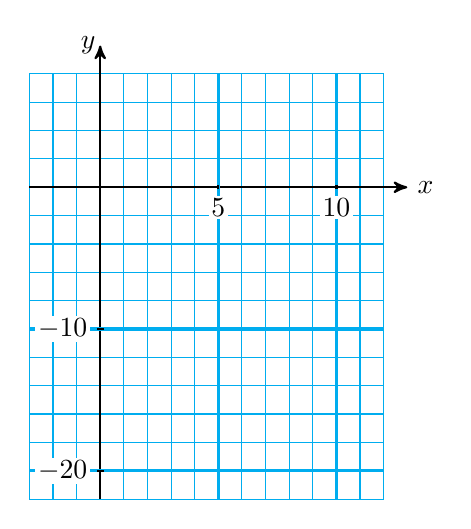
\begin{tikzpicture}[xscale=.3, yscale=.18]
\draw[cyan] (-3,-22) grid[ystep=2] (12,8);
\draw[black, thick, ->, >=stealth'] (-3,0)--(13,0) node[right]{$x$};
\draw[black, thick, ->, >=stealth'] (0,-22)--(0,10) node[left, xshift=2]{$y$};
\foreach \x in {5,10} {
 \draw[cyan, very thick] (\x,-22)--++(0,30);
 \draw[black, thick] (\x,.15) --++(0,-.3) node[below, yshift=-2, fill=white, inner sep=1]   {$\x$};
}
\foreach \x  in  {-10,-20} {
 \draw[cyan, very thick] (-3,\x)--++(15,0);
\draw[black, thick] (.15,\x) --++(-.3,0) node[left, xshift=-2, fill=white, inner sep=1]   {$\x$};
}
\end{tikzpicture}
\newline


cr6-43ans

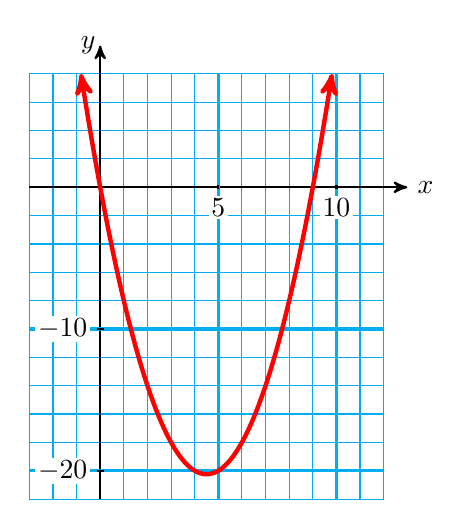
\begin{tikzpicture}[xscale=.3, yscale=.18]
\draw[cyan] (-3,-22) grid[ystep=2] (12,8);
\draw[black, thick, ->, >=stealth'] (-3,0)--(13,0) node[right]{$x$};
\draw[black, thick, ->, >=stealth'] (0,-22)--(0,10) node[left, xshift=2]{$y$};
\foreach \x in {5,10} {
 \draw[cyan, very thick] (\x,-22)--++(0,30);
 \draw[black, thick] (\x,.15) --++(0,-.3) node[below, yshift=-2, fill=white, inner sep=1]   {$\x$};
}
\foreach \x  in  {-10,-20} {
 \draw[cyan, very thick] (-3,\x)--++(15,0);
\draw[black, thick] (.15,\x) --++(-.3,0) node[left, xshift=-2, fill=white, inner sep=1]   {$\x$};
}
\draw[samples=65,domain={-sqrt(113)/2+4.5}:{sqrt(113)/2+4.5},smooth,variable=\x,red, ultra thick, <->, >=stealth'] plot ({\x},{(\x)^2-9*\x});
\end{tikzpicture}
\newline


cr6-45ans

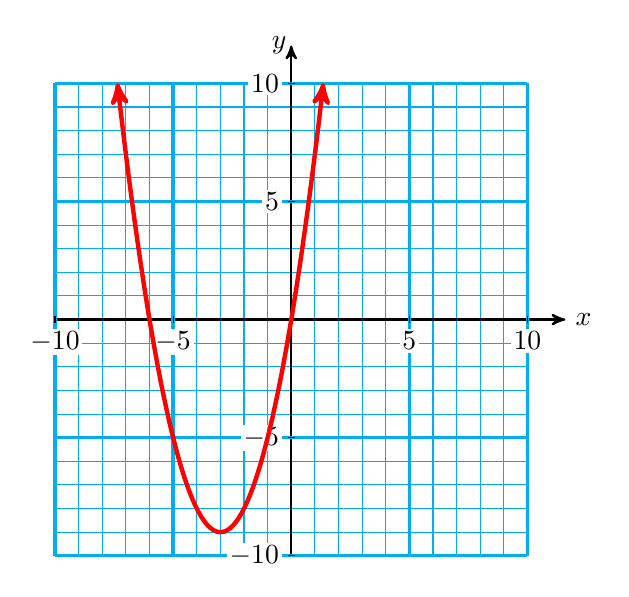
\begin{tikzpicture} [scale=.3]
\coordinate (O) at (0,0);
\draw[cyan] (-10,-10) grid (10,10);
\draw[black,thick, ->, >=stealth'] (-10,0)--(11.6,0) node[right]{$x$};
\draw[black,thick, ->, >=stealth'] (0,-10)--(0,11.6) node[left, xshift=2]{$y$};
\foreach \x in  {-5, 5, -10, 10} {
 \draw[cyan, very thick] (\x,-10) --++(0,20);
 \draw[cyan, very thick] (-10,\x) --++(20,0);
 \draw[black] (\x,.15) --++(0,-.3)  node[below, yshift=-2, fill=white, inner sep=1]   {$\x$};
 \draw[black] (.15,\x) --++(-.3,0)  node[left, xshift=-2, fill=white, inner sep=1]   {$\x$};
}
\draw[samples=65,domain={-sqrt(19)-3}:{sqrt(19)-3},smooth,variable=\x,red, ultra thick, <->, >=stealth'] plot ({\x},{(\x)^2+6*\x});
\end{tikzpicture}
\newline


cr6-47 triangle

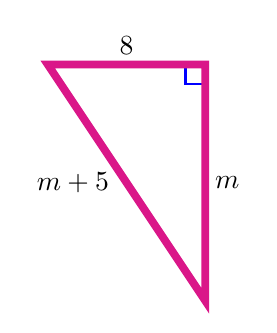
\begin{tikzpicture}
\draw[blue,thick] (0,0) rectangle ++(-.25,-.25);
\draw[magenta!90!black, line width=1mm] (0,0)--(-2,0)--(0,-3)--cycle;
\node[left] at (-1.1,-1.5) {$m+5$};
\node[right] at (0,-1.5) {$m$};
\node[above] at (-1,0) {$8$};
\end{tikzpicture}
\newline


cr6-48 triangle

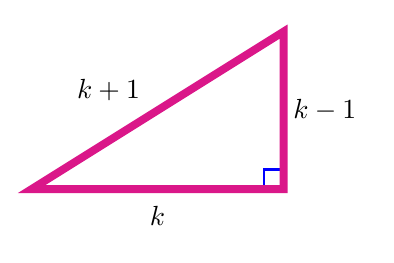
\begin{tikzpicture}
\draw[blue,thick] (0,0) rectangle ++(-.25,.25);
\draw[magenta!90!black, line width=1mm] (0,0)--(-3.2,0)--(0,2)--cycle;
\node[right] at (0,1) {$k-1$};
\node[below] at (-1.6,-0.1) {$k$};
\node[above left] at (-1.7,1) {$k+1$};
\end{tikzpicture}
\newline





\section{Other stuff}

10 by 10 grid: hp-2-3-12

8 by 8 grid: hp-4-5-17

5-by-5 grid hp-6-4-9



\end{document}
